\paragraph{Write a little computer program that sums up $N$ random numbers 
drawn from $[-1,1]$. Divide by $N$ and compare the obtained distribution to the 
Gaussian distribution, for $N=10,100,1000$, by plotting the histogram and the 
appropriate analytical function together.} \ \\
\\ 
To create a distribution we run a loop for 1000 iterations, at each iteration 
we create a random number by summing up $N$ number between -1 and 1.
The computer program can be implemented using the following python snippet: \\
\begin{lstlisting}
import random

import matplotlib.pyplot as plt
import numpy as np
from scipy.optimize import curve_fit

M = 1000
for N in [10, 100, 1000]:
    rs = []
    for _ in range(M):
        r = 0
        for i in range(N):
            r += random.uniform(-1, 1)
        rs.append(r / N)

    plt.figure(figsize=(3, 3))
    plt.xlim(-0.6, 0.6)
    plt.ylim(0, 130)
    plt.hist(rs, bins=20)
    plt.savefig(f'../figures/{N}.pdf')
\end{lstlisting}
This leads to these plots:
\begin{figure}[h!]
    \centering
    \begin{minipage}{.3\linewidth}
      \centering
      \subfloat[$N=10$]{
        \label{:a}
        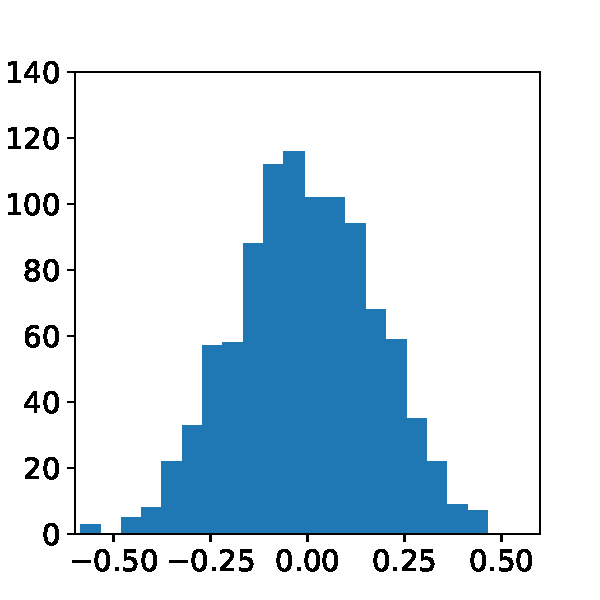
\includegraphics[scale=.5]{./figures/10.pdf}
      }
    \end{minipage}%
    \begin{minipage}{.3\linewidth}
      \centering
      \subfloat[$N=100$]{
        \label{:b}
        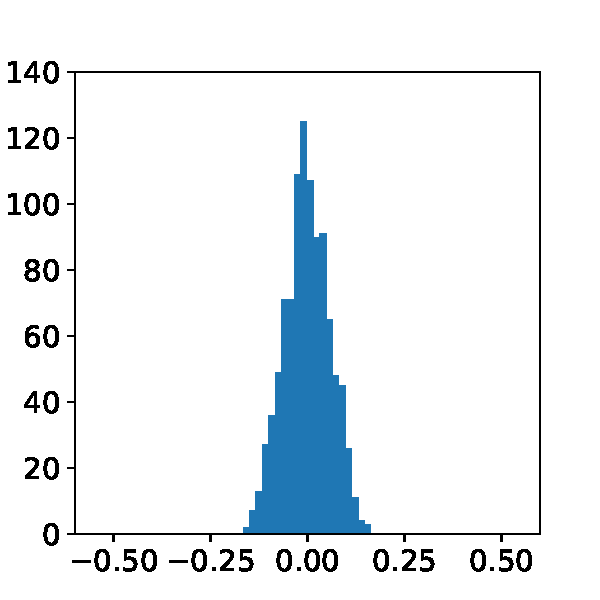
\includegraphics[scale=.5]{./figures/100.pdf}
      }
    \end{minipage}
    \begin{minipage}{.3\linewidth}
      \centering
      \subfloat[$N=1000$]{
        \label{:b}
        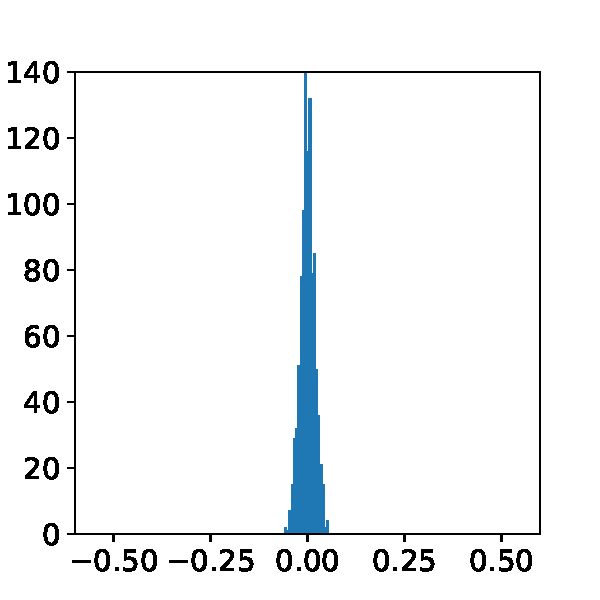
\includegraphics[scale=.5]{./figures/1000.pdf}
      }
    \end{minipage}
\end{figure} \ \\
As is to be expected, the expectation value of the distrition does not change 
with increasing $N$, but stays constant at $\approx0$. The width of the 
curve decreases for a large number of summands. This is due to the fact that 
we divide the sum by $N$.
